\documentclass{article}
\usepackage{tikz}
\usetikzlibrary{arrows.meta}
\usetikzlibrary{shapes.geometric}

\tikzset{
  database/.pic = {
    \coordinate (-top) at (0,0.5);
    \coordinate (-top-center) at (0,0);
    \draw (0,0) ellipse (1 and 0.5);
    \draw (-1,0) -- (-1,-2);
    \draw (-1,-2) arc (180:360:1 and 0.5);
    %\draw [dashed] (-1,-2) arc (180:360:1 and -0.5);
    \draw (1,-2) -- (1, 0);
    \fill [gray,opacity=0.5] (-1,0) -- (-1,-2) arc (180:360:1 and 0.5) -- (1,0) arc (0:180:1 and -0.5);
  }
}

\begin{document}

Case 1: Fully Synchronized
\\[12pt]

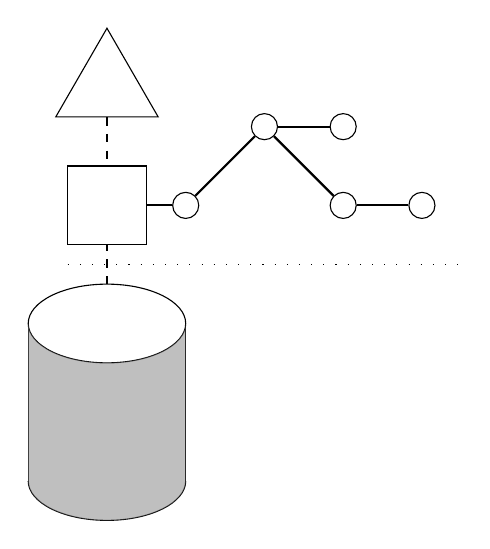
\begin{tikzpicture}[scale=0.5]
  \node[draw,regular polygon,regular polygon sides=3,minimum size=1.5cm] (pf-sl) at (0,5) {};
  \node[draw,rectangle,minimum size=1cm] (pf-root) at (0,2) {};
  \draw[dashed] (pf-sl) -- (pf-root);

  \node[draw,circle] (pf-n1) at (2,2) {};
  \node[draw,circle] (pf-n2) at (4,4) {};
  \node[draw,circle] (pf-n3) at (6,4) {};
  \node[draw,circle] (pf-n4) at (6,2) {};
  \node[draw,circle] (pf-n5) at (8,2) {};
  \draw[thick] (pf-root) -- (pf-n1);
  \draw[thick] (pf-n1) -- (pf-n2);
  \draw[thick] (pf-n2) -- (pf-n3);
  \draw[thick] (pf-n2) -- (pf-n4);
  \draw[thick] (pf-n4) -- (pf-n5);

  \pic (p-root) at (0,-1) {database};
  \draw[dashed] (p-root-top) -- (pf-root);

  \draw[loosely dotted] (-1,0.5) -- (9,0.5);
\end{tikzpicture}

Case 2: Fast Forward
\\[12pt]

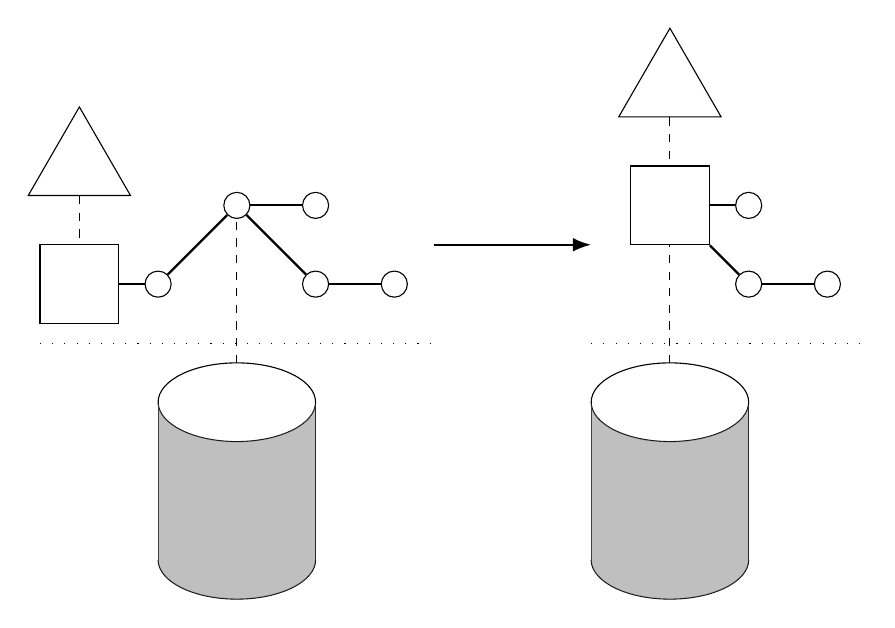
\begin{tikzpicture}[scale=0.5]
  \node[draw,regular polygon,regular polygon sides=3,minimum size=1.5cm] (pf-sl) at (0,5) {};
  \node[draw,rectangle,minimum size=1cm] (pf-root) at (0,2) {};
  \draw[dashed] (pf-sl) -- (pf-root);

  \node[draw,circle] (pf-n1) at (2,2) {};
  \node[draw,circle] (pf-n2) at (4,4) {};
  \node[draw,circle] (pf-n3) at (6,4) {};
  \node[draw,circle] (pf-n4) at (6,2) {};
  \node[draw,circle] (pf-n5) at (8,2) {};
  \draw[thick] (pf-root) -- (pf-n1);
  \draw[thick] (pf-n1) -- (pf-n2);
  \draw[thick] (pf-n2) -- (pf-n3);
  \draw[thick] (pf-n2) -- (pf-n4);
  \draw[thick] (pf-n4) -- (pf-n5);

  \pic (p-root) at (4,-1) {database};
  \draw[dashed] (p-root-top) -- (pf-n2);

  \draw[loosely dotted] (-1,0.5) -- (9,0.5);

  \draw[thick,-Latex] (9, 3) -- (13, 3);

  \node[draw,regular polygon,regular polygon sides=3,minimum size=1.5cm] (pf2-sl) at (15,7) {};
  \node[draw,rectangle,minimum size=1cm] (pf2-root) at (15,4) {};
  \draw[dashed] (pf2-sl) -- (pf2-root);

  \node[draw,circle] (pf2-n3) at (17,4) {};
  \node[draw,circle] (pf2-n4) at (17,2) {};
  \node[draw,circle] (pf2-n5) at (19,2) {};
  \draw[thick] (pf2-root) -- (pf2-n3);
  \draw[thick] (pf2-root) -- (pf2-n4);
  \draw[thick] (pf2-n4) -- (pf2-n5);

  \pic (p2-root) at (15,-1) {database};
  \draw[dashed] (p2-root-top) -- (pf2-root);
  \draw[loosely dotted] (13,0.5) -- (20,0.5);
\end{tikzpicture}

Case 3: Bootstrap Required
\\[12pt]

\end{document}
